% !Mode:: "TeX:UTF-8"
% !TEX program  = xelatex

%\documentclass{cumcmthesis}
\documentclass[withoutpreface,bwprint]{cumcmthesis} %去掉封面与编号页

\usepackage{url}   % 网页链接
\usepackage{subcaption} % 子标题
\title{全国大学生数学建模竞赛编写的 \LaTeX{} 模板}
\tihao{A}
\baominghao{4321}
\schoolname{XX大学}
\membera{}
\memberb{向左}
\memberc{哈哈}
\supervisor{老师}
\yearinput{2017}
\monthinput{08}
\dayinput{22}

\title{微分方程数值解第三周第二次作业}
\begin{document}
	\maketitle
	~\\
	~\\
	
	作业:
	
	$$
	\left\{
	\begin{array}{lcl}
	-\dfrac{d}{dx}(x\dfrac{du}{dx})+\dfrac{du}{dx}+u=e^{x}(2xsin(x)+cosx). &, &0 \leq x \leq 1\\
	u(0)=1,u(1)=ecos(1) \\
	\end{array}
	\right.
	$$
	
	该问题的精确解为$ u(x)=e^{x}cosx $.
	
	定义误差为$ E_{\infty}(N)=\max \limits_{0 \leq i \leq N}|u(x_{i}-u_i)| $,$N$为区间个数。
	
	要求用直接差分法求出上述例子的数值解 求出不同步长下误差的变化,通过图形和表格总结在步长变化时有什么规律。
	~\\
	~\\
	解:本题的差分格式为
	
	\begin{equation*}
	\begin{split}
		&\dfrac{-1}{h_{i}+h_{i+1}}(\dfrac{2x_{i-\frac{1}{2}}}{h_{i}}+1)u_{i-1}+\\
		&\dfrac{1}{h_{i}+h_{i+1}}[\dfrac{2x_{i+\frac{1}{2}}}{h_{i+1}}+\dfrac{2x_{i-\frac{1}{2}}}{h_{i}}+(h_{i}+h_{i+1})]u_{i}+\\
		&\dfrac{-1}{h_{i}+h_{i+1}}(\dfrac{2x_{i+\frac{1}{2}}}{h_{i+1}}-1)u_{i+1}\\
		&=e^{x_{i}}(2x_{i}sin(x_{i})cos(x_{i}))
	\end{split}
	\end{equation*}
	
	其中,$ 1 \leq i \leq N-1 $,$ u_{0}=1,u_{N}=ecos(1) $.
	
	系数矩阵为$ Au=f $
	
	$$
	A=
	\begin{bmatrix}
	\frac{1}{h_{1}+h_{2}}(\dfrac{2x_{1+\frac{1}{2}}}{h_{2}}+\dfrac{2x_{1-\frac{1}{2}}}{h_{1}})+1  & -\frac{1}{h_{1}+h_{2}}(\dfrac{2x_{1+\frac{1}{2}}}{h_{2}}-1)  \\


	 -\frac{1}{h_{2}+h_{3}}(\dfrac{2x_{2-\frac{1}{2}}}{h_{2}}+1) &  \frac{1}{h_{2}+h_{3}}(\dfrac{2x_{2+\frac{1}{2}}}{h_{3}}+\dfrac{2x_{2-\frac{1}{2}}}{h_{2}})+1 &  -\frac{1}{h_{2}+h_{3}}(\dfrac{2x_{2+\frac{1}{2}}}{h_{3}}-1)\\
	 
	 \ddots & \ddots &\ddots\\
	 
	\end{bmatrix}
	$$ 
	
	为三对角矩阵。
	
	$$
	f=
	[f_{1}+\frac{1}{h_{1}+h_{2}}(\dfrac{2x_{1-\frac{1}{2}}}{h_{1}}+1),f2,\cdots,f_{N-1}+\frac{1}{h_{N-1}+h_{N}}(\dfrac{2x_{N-\frac{1}{2}}}{h_{N}}-1)ecos(1)]^{T}
	$$
	
	$$f_{i}=e^{x_{i}}(2x_{i}sin(x_{i})+cos(x_{i}))$$.
	$$u=[u_{1},u_{2},\cdots,u_{N-1}]^{T}$$
	
	解题程序运行于Matlab 2018a.
	
	设k为步长系数,$h_{i}=k h_{i-1}$,如果将区间划分成N个小区间,h1为第一个区间的步长,则有$h1+h1k+h1k^{2}+h1k^{3}+\cdots +h1k^{N-1}==1$,可以解出
	
	$$h1=\dfrac{1-k}{1-k^{N}}$$,
	因此取定N和k时步长可以确定。
	
	当取N=64,k分别取0.95、1和1.05时,直接差分的数值解和精确解对比见图\ref{fig:f1},图\ref{fig:f2}和图\ref{fig:f3},可以发现,数值解都接近于数值解。
	\begin{figure}
	\centering
	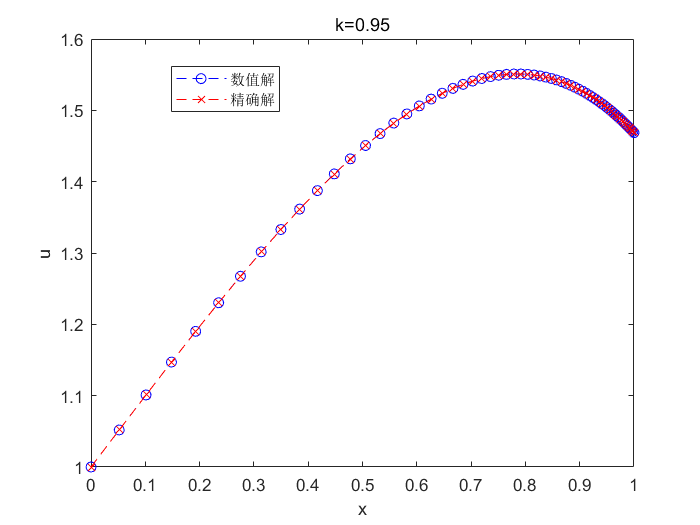
\includegraphics[width=0.7\linewidth]{figures/f1}
	\caption{k=0.95}
	\label{fig:f1}
	\end{figure}
	
	\begin{figure}
	\centering
	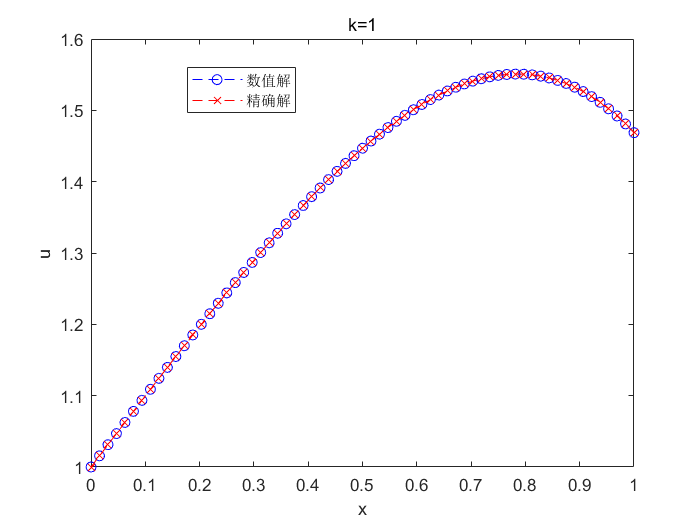
\includegraphics[width=0.7\linewidth]{figures/f2}
	\caption{k=1}
	\label{fig:f2}
	\end{figure}
	
	\begin{figure}
	\centering
	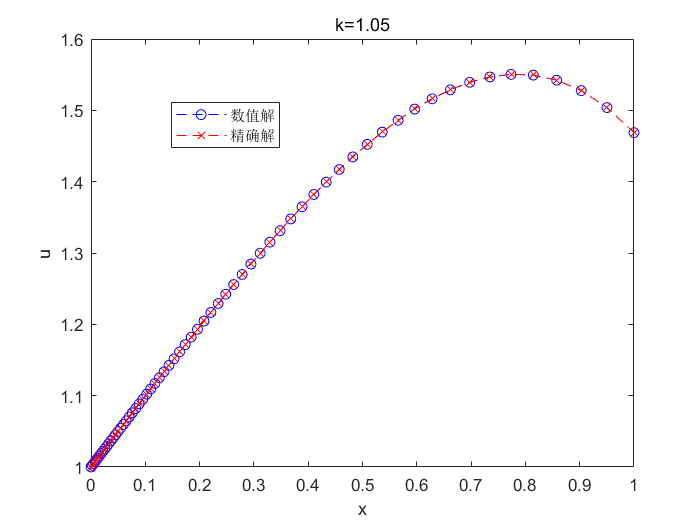
\includegraphics[width=0.7\linewidth]{figures/f3}
	\caption{k=1.05}
	\label{fig:f3}
	\end{figure}
	
	
	此时的误差曲线见图\ref{fig:f4},k=1时,即等步长时,数值解的误差最小。
	\begin{figure}
	\centering
	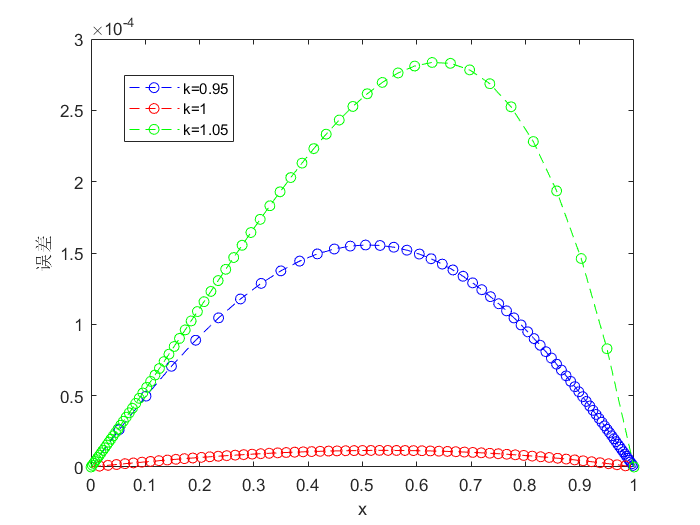
\includegraphics[width=0.7\linewidth]{figures/f4}
	\caption{不同步长系数下数值解的误差}
	\label{fig:f4}
	\end{figure}
	
	定义误差阶
	$$rate=\log{2}{\dfrac{E_{\infty}(N)}{E_{\infty}(2N)}}$$.
	
	算出不同步长系数对应不同区间数的误差阶,得到表\ref{tab:1},可以发现只有当等步长时,才能达到二阶精度。
	% Table generated by Excel2LaTeX from sheet 'Sheet1'
	\begin{table}[htbp]
	\centering
	\caption{误差和误差阶}
	\begin{tabular}{cccc}
	\toprule[1.5pt]
	k     & N     & \multicolumn{1}{l}{$E_{\infty}(N)$} & \multicolumn{1}{l}{$E_{\infty}(N)/E_{\infty}(2N)$} \\
	\multirow{5}[0]{*}{0.95} & 8     & 2.63E-04 & \multicolumn{1}{c}{*} \\
	& 16    & 2.99E-04 & -0.18289 \\
	& 32    & 2.07E-04 & 0.531652 \\
	& 64    & 1.56E-04 & 0.410649 \\
	& 128   & 1.45E-04 & 0.10114 \\
	\hline
	\multirow{5}[0]{*}{1} & 8     & 7.41E-04 & \multicolumn{1}{c}{*} \\
	& 16    & 1.86E-04 & 1.995669 \\
	& 32    & 4.65E-05 & 1.996735 \\
	& 64    & 1.16E-05 & 2.000042 \\
	& 128   & 2.91E-06 & 1.999751 \\
	\hline
	\multirow{5}[0]{*}{1.05} & 8     & 1.78E-03 & \multicolumn{1}{c}{*} \\
	& 16    & 7.56E-04 & 1.23785 \\
	& 32    & 3.99E-04 & 0.923133 \\
	& 64    & 2.84E-04 & 0.491326 \\
	& 128   & 2.62E-04 & 0.114149 \\
	\bottomrule[1.5pt]
	\end{tabular}%
	\label{tab:1}%
	\end{table}%

	
\end{document}